\section{IDF Version Updater}\label{idf-version-updater}

The transition programs have been written as console applications similar to EnergyPlus. However, that may not be the easiest for users who want to transition several versions or several files at one time. Thus the IDF Version Updater GUI application was created.

The IDF Version Updater lives in the folder with the multiple transition programs -- see Figure~\ref{fig:transition-gui-screen}. Note that this application is also available from the EP-Launch Utilities tab (utility: IDFVersionUpdater). If you need to convert files from older than V6.0, the transition program set will need to be downloaded before use. Once ``IDF Version Updater'' is selected from the Utilities pulldown list, click on the ``Run IDF Version Updater'' box and the single window shown below appears:

\begin{figure}[hbtp] % fig 29
\centering
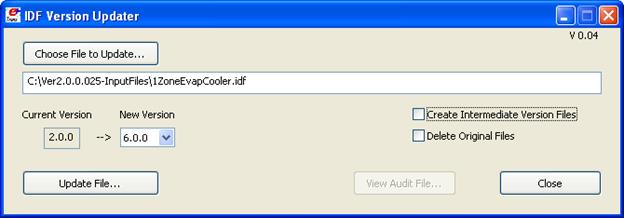
\includegraphics[width=0.9\textwidth, height=0.9\textheight, keepaspectratio=true]{media/image027.jpg}
\caption{Transition GUI screen \protect \label{fig:transition-gui-screen}}
\end{figure}

Using the program is quite simple. As the window indicates, you press ``Choose File to Update'' to select a file or list of files (see IDF Version Converter / Transition File Lists) to convert. If doing multiple transitions using a transition file list you also press the ``Choose File to Update, a browse window will appear at the bottom of which is a pulldown list for the''Files of Type``. Select the''Text File With List of EnergyPlus Files (*.lst)" (see the section IDF Version Converter / Transition File Lists for format of this .lst file) option. Once a file is found, its version is checked and appears as the ``Current Version''. By default, the latest ``New Version'' will be selected by the program - you can override this by choosing a different file version as the end version. The ``Update File'' button will then be able to be selected and the conversion will be done. The audit from the multiple transitions will be able to be viewed once the process is complete. If you are doing multiple transitions (e.g., from V2.2 to V6), you can select the check box ``Create Intermediate Files'' and after each transition, a file for the resultant version will be created and labeled \textless{}filename\textgreater{})\_Vx.idf (where x is an abbreviated version number).

The converted file becomes the new \textless{}file\textgreater{}.idf and the original file is saved in the original folder as \textless{}file\textgreater{}\_original.idf. To delete the original file instead of saving it, check the ``Delete Original Files'' checkbox.

% table 27
\begin{longtable}[c]{p{2.5in}p{3.5in}}
\caption{IDF Version Updater Output Files and Descriptions. \label{table:idf-version-updater-output-files}} \tabularnewline
\toprule 
Transition Output File Name & Description \tabularnewline
\midrule
\endfirsthead

\caption[]{IDF Version Updater Output Files and Descriptions.} \tabularnewline
\toprule 
Transition Output File Name & Description \tabularnewline
\midrule
\endhead

< filename > \_Transition.audit & This is the contents of what you would see on the screen if you sat and watched the transition process during a console run. If you convert multiple versions, all the messages are shown in this file. \tabularnewline
< filename > .idf & Converted results to the latest version or version selected. \tabularnewline
< filename > \_Vxxx.idf & If you don't select "create intermediate versions", this will only be the original version. Otherwise will have each version. \tabularnewline
\bottomrule
\end{longtable}
